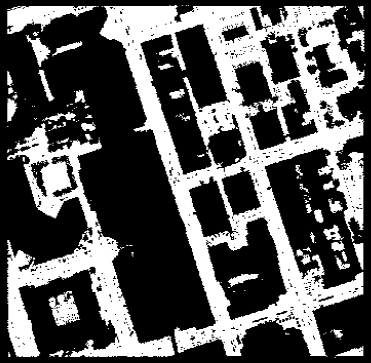
\includegraphics[height=3cm]{figure/Chapter6/高程约束提取道路点}
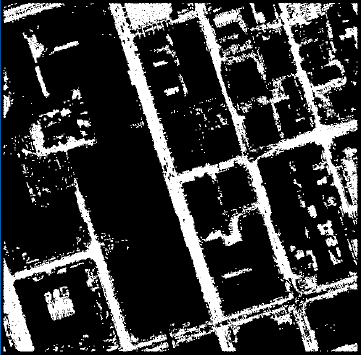
\includegraphics[height=3cm]{figure/Chapter6/强度约束提取道路点}
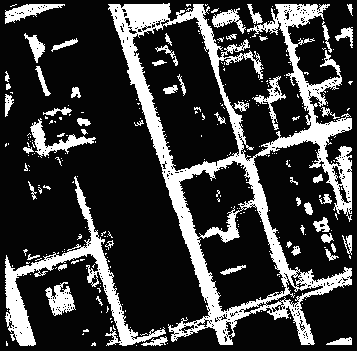
\includegraphics[height=3cm]{figure/Chapter6/条带优化处理}
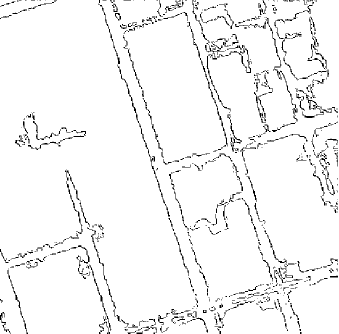
\includegraphics[height=3cm]{figure/Chapter6/道路轮廓线自适应提取}
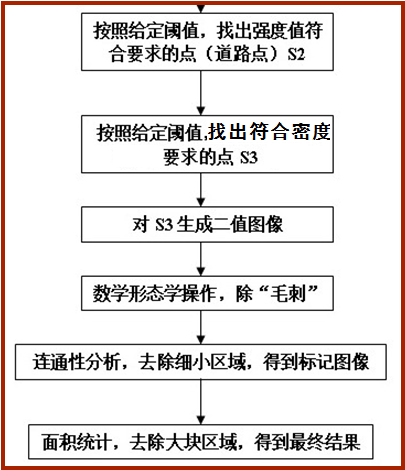
\includegraphics[width=0.3\linewidth]{figure/Chapter6/相位编码圆盘步骤2}
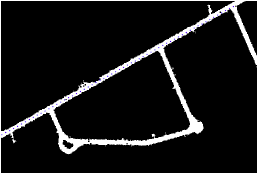
\includegraphics[height=3cm]{figure/Chapter6/路段灰度图}
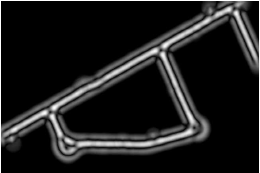
\includegraphics[height=3cm]{figure/Chapter6/路段幅度图}
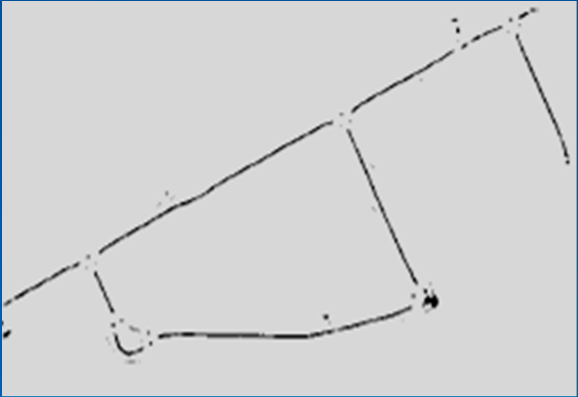
\includegraphics[height=3cm]{figure/Chapter6/道路中心线段}
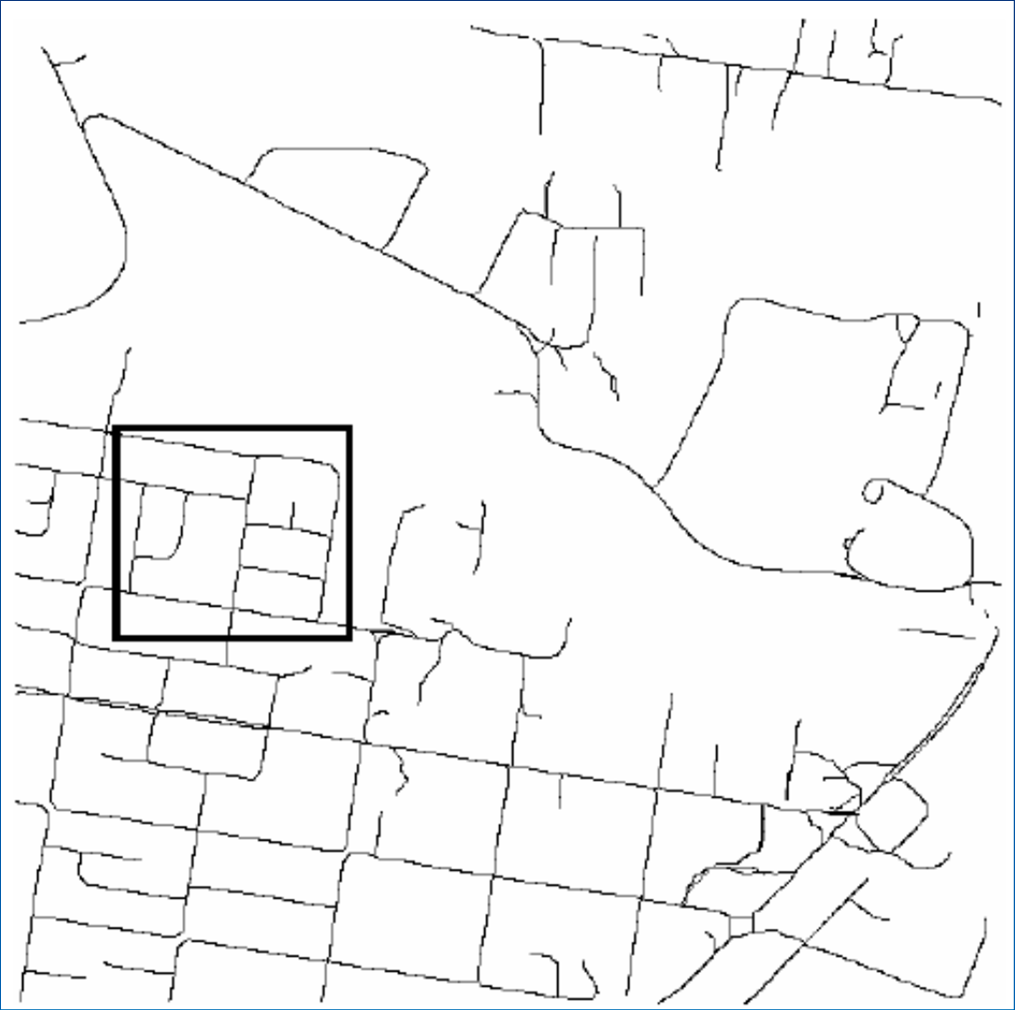
\includegraphics[width=0.4\linewidth]{figure/Chapter6/卷及处理得到的道路中心线}
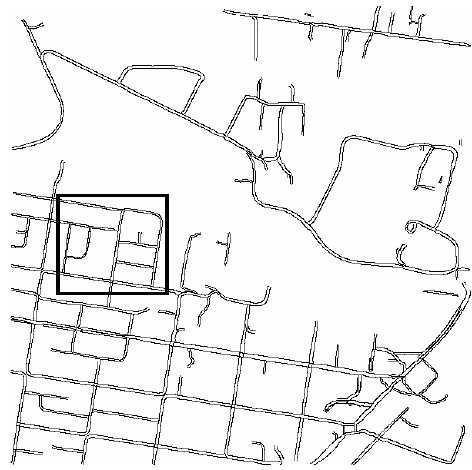
\includegraphics[width=0.4\linewidth]{figure/Chapter6/卷积处理得到的道路轮廓线}
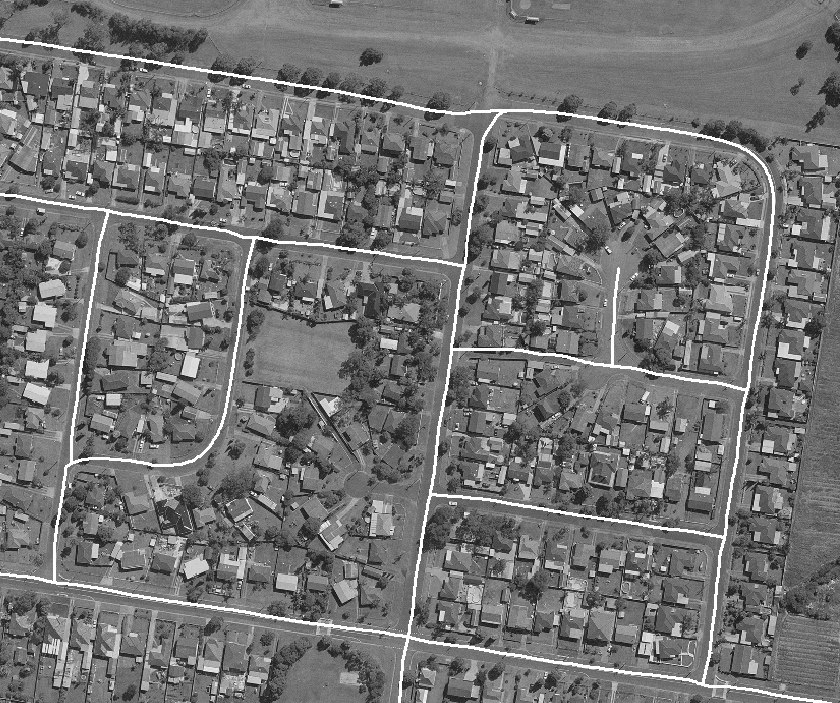
\includegraphics[width=0.4\linewidth]{figure/Chapter6/道路中心线与影像的叠加效果}
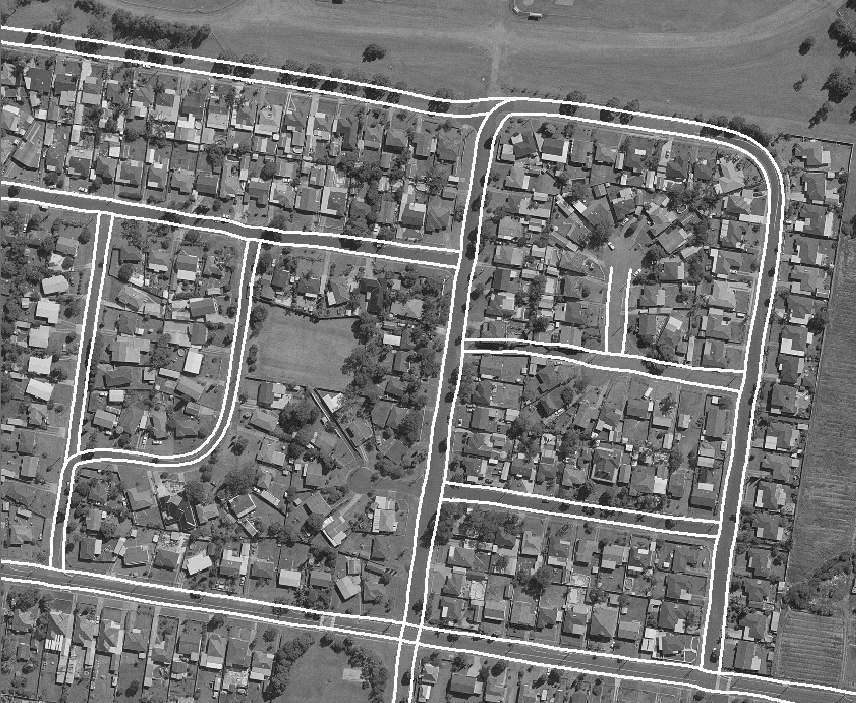
\includegraphics[width=0.4\linewidth]{figure/Chapter6/道路轮廓线与影像的叠加效果}
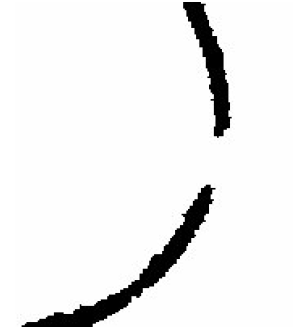
\includegraphics[width=0.4\linewidth]{figure/Chapter6/提取道路不连续}
